\section{Results}

\subsection{Model Comparison}

The initial model comparison evaluated KNN, Decision Tree, Random Forest, SVM,
and Naive Bayes using stratified 5-fold cross-validation. The same
preprocessing workflow was applied inside each fold to reduce the risk of data
leakage. At this stage, no dimensionality-reduction or balancing strategy was
applied, establishing a baseline for the subsequent preprocessing experiments.

Random Forest obtained the best overall performance among the evaluated
classifiers, with overall accuracy of 0.9950 and macro-F1 of 0.9945. Because
the encoded labels map \texttt{ckd} to 0 and \texttt{notckd} to 1, the
class-wise metrics were reported explicitly instead of relying only on the
default positive class used by scikit-learn. For CKD, Random Forest obtained
precision of 0.9922, recall of 1.0000, and F1-score of 0.9961; for NOTCKD, it
obtained precision of 1.0000, recall of 0.9861, and F1-score of 0.9930.

SVM and Naive Bayes also performed well, but Random Forest achieved the
strongest overall metric profile. These results address the first objective of
the study by showing that Random Forest was the best-performing classifier
among the evaluated supervised learning models. For this reason, it was used as
the reference model in the balancing, dimensionality-reduction, optimization,
and interpretability stages. Table~\ref{tab:model_comparison} summarizes the
main metrics, while Figure~\ref{fig:model_comparison_results} presents the
F1-score distribution and ROC curves.

\begin{table}[!htbp]
\centering
\caption{Initial classifier comparison using no dimensionality reduction and no balancing.}
\label{tab:model_comparison}
\begin{tabular}{lcccc}
\hline
Model & Accuracy & Macro-F1 & CKD F1 & NOTCKD F1 \\
\hline
Random Forest & 0.9950 & 0.9945 & 0.9961 & 0.9930 \\
SVM & 0.9749 & 0.9732 & 0.9799 & 0.9664 \\
Decision Tree & 0.9598 & 0.9567 & 0.9683 & 0.9452 \\
Naive Bayes & 0.9548 & 0.9522 & 0.9633 & 0.9412 \\
KNN & 0.9447 & 0.9419 & 0.9547 & 0.9290 \\
\hline
\end{tabular}
\end{table}

\begin{figure}[!htbp]
\centering
\begin{subfigure}{0.48\linewidth}
\centering
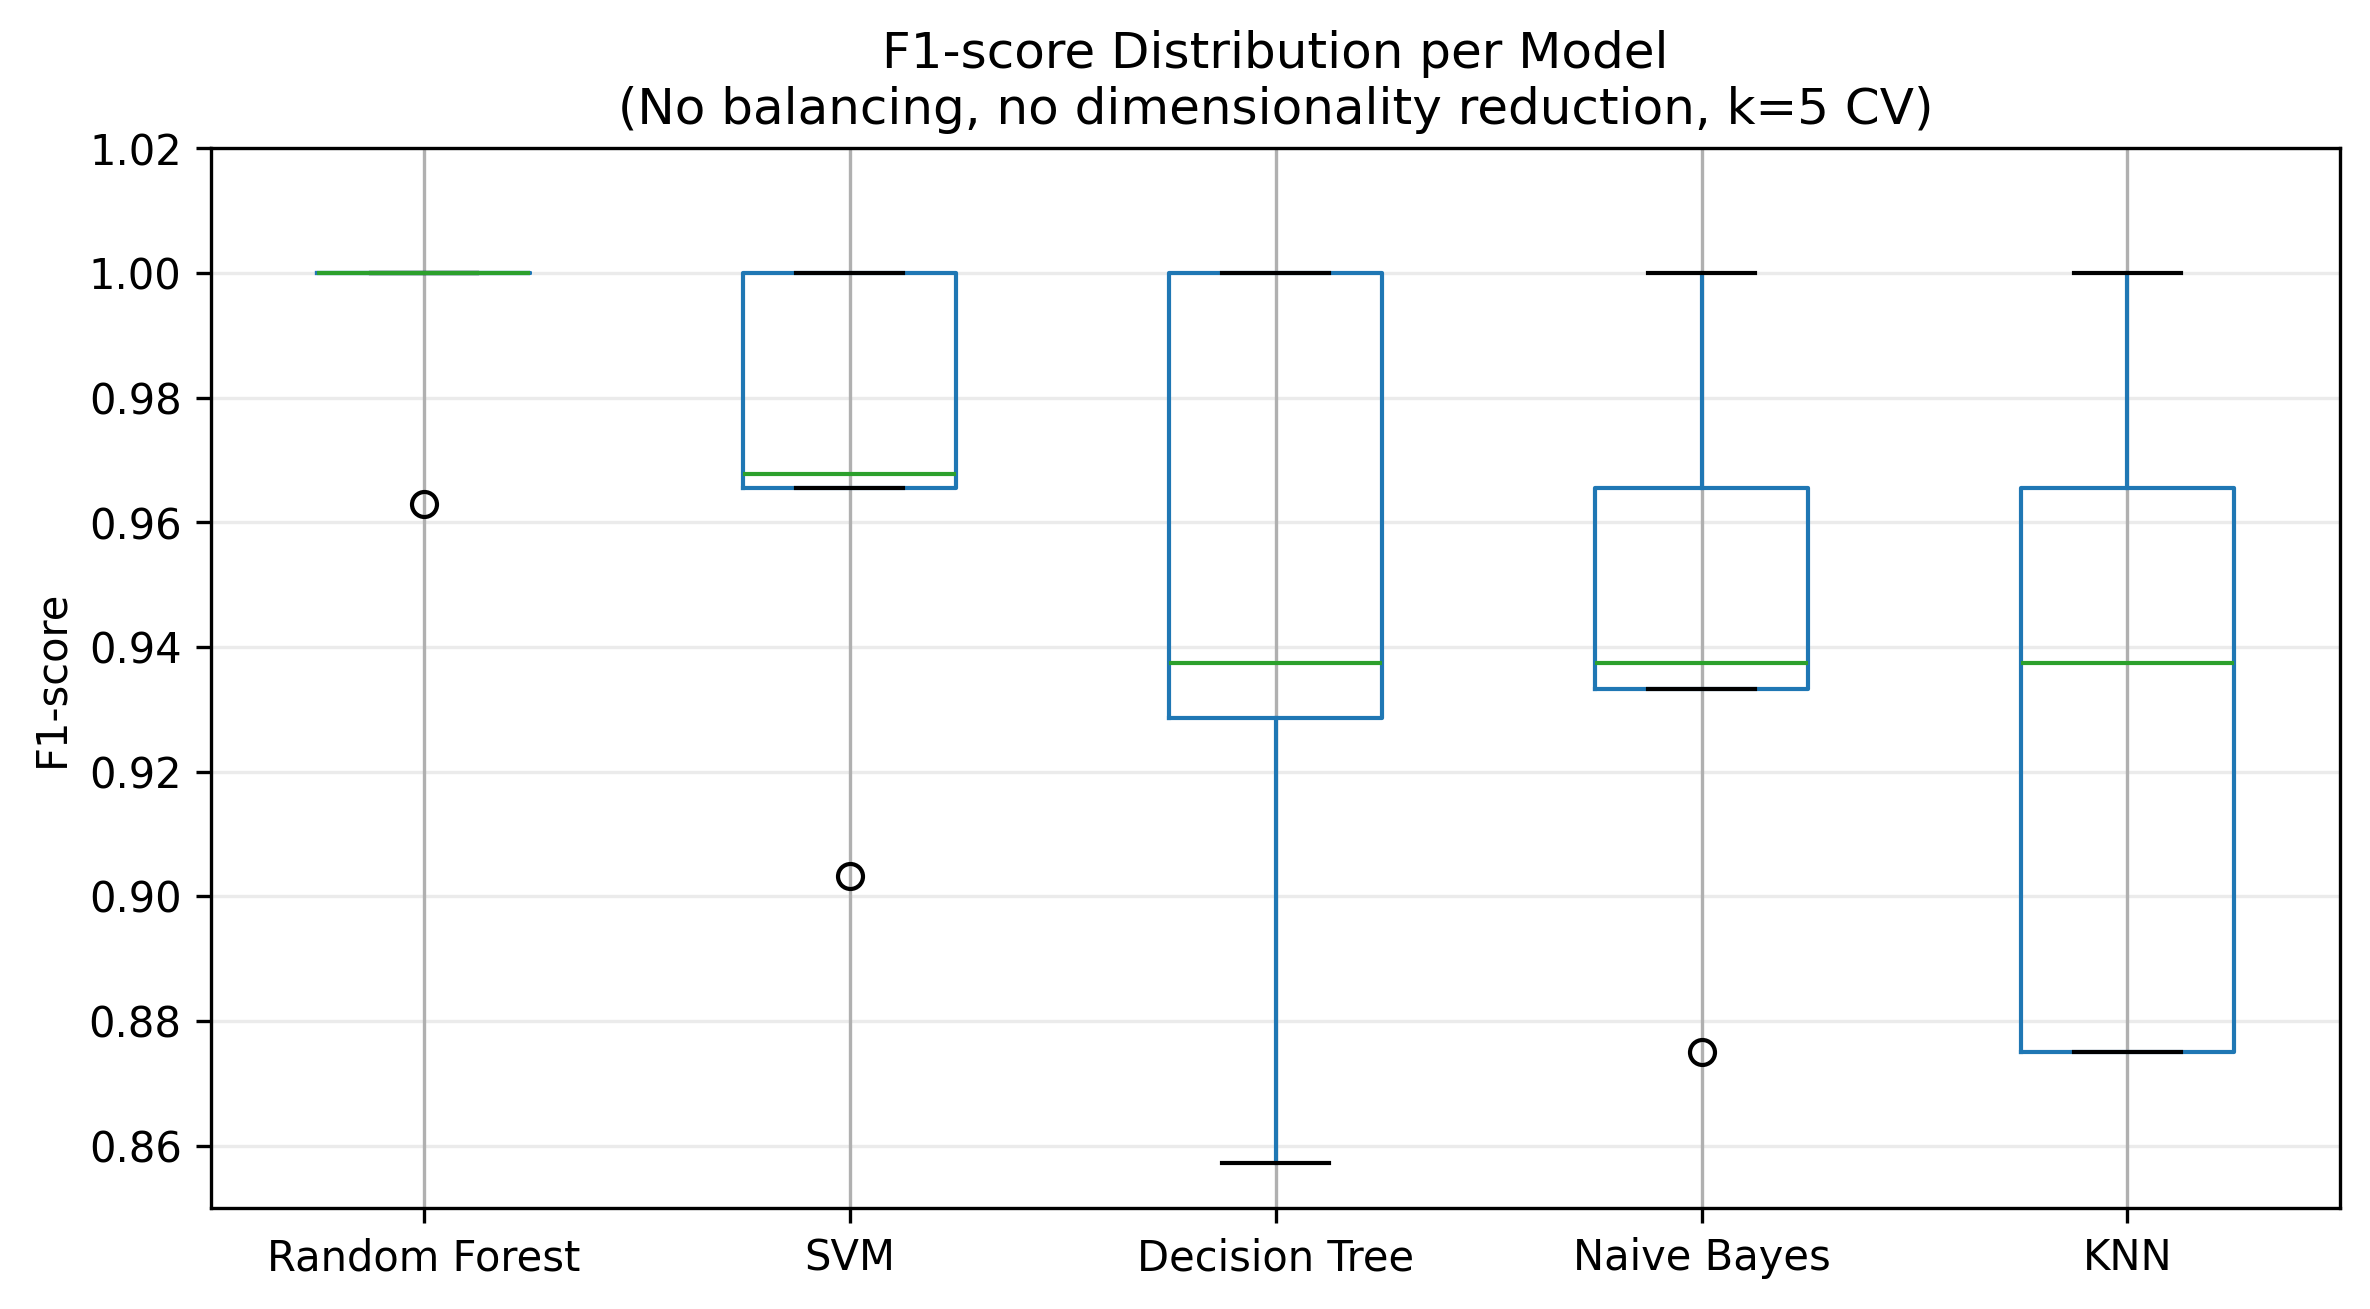
\includegraphics[width=\linewidth]{figures/model_comparison_no_dr_boxplot.png}
\caption{F1-score distribution.}
\end{subfigure}
\hfill
\begin{subfigure}{0.48\linewidth}
\centering
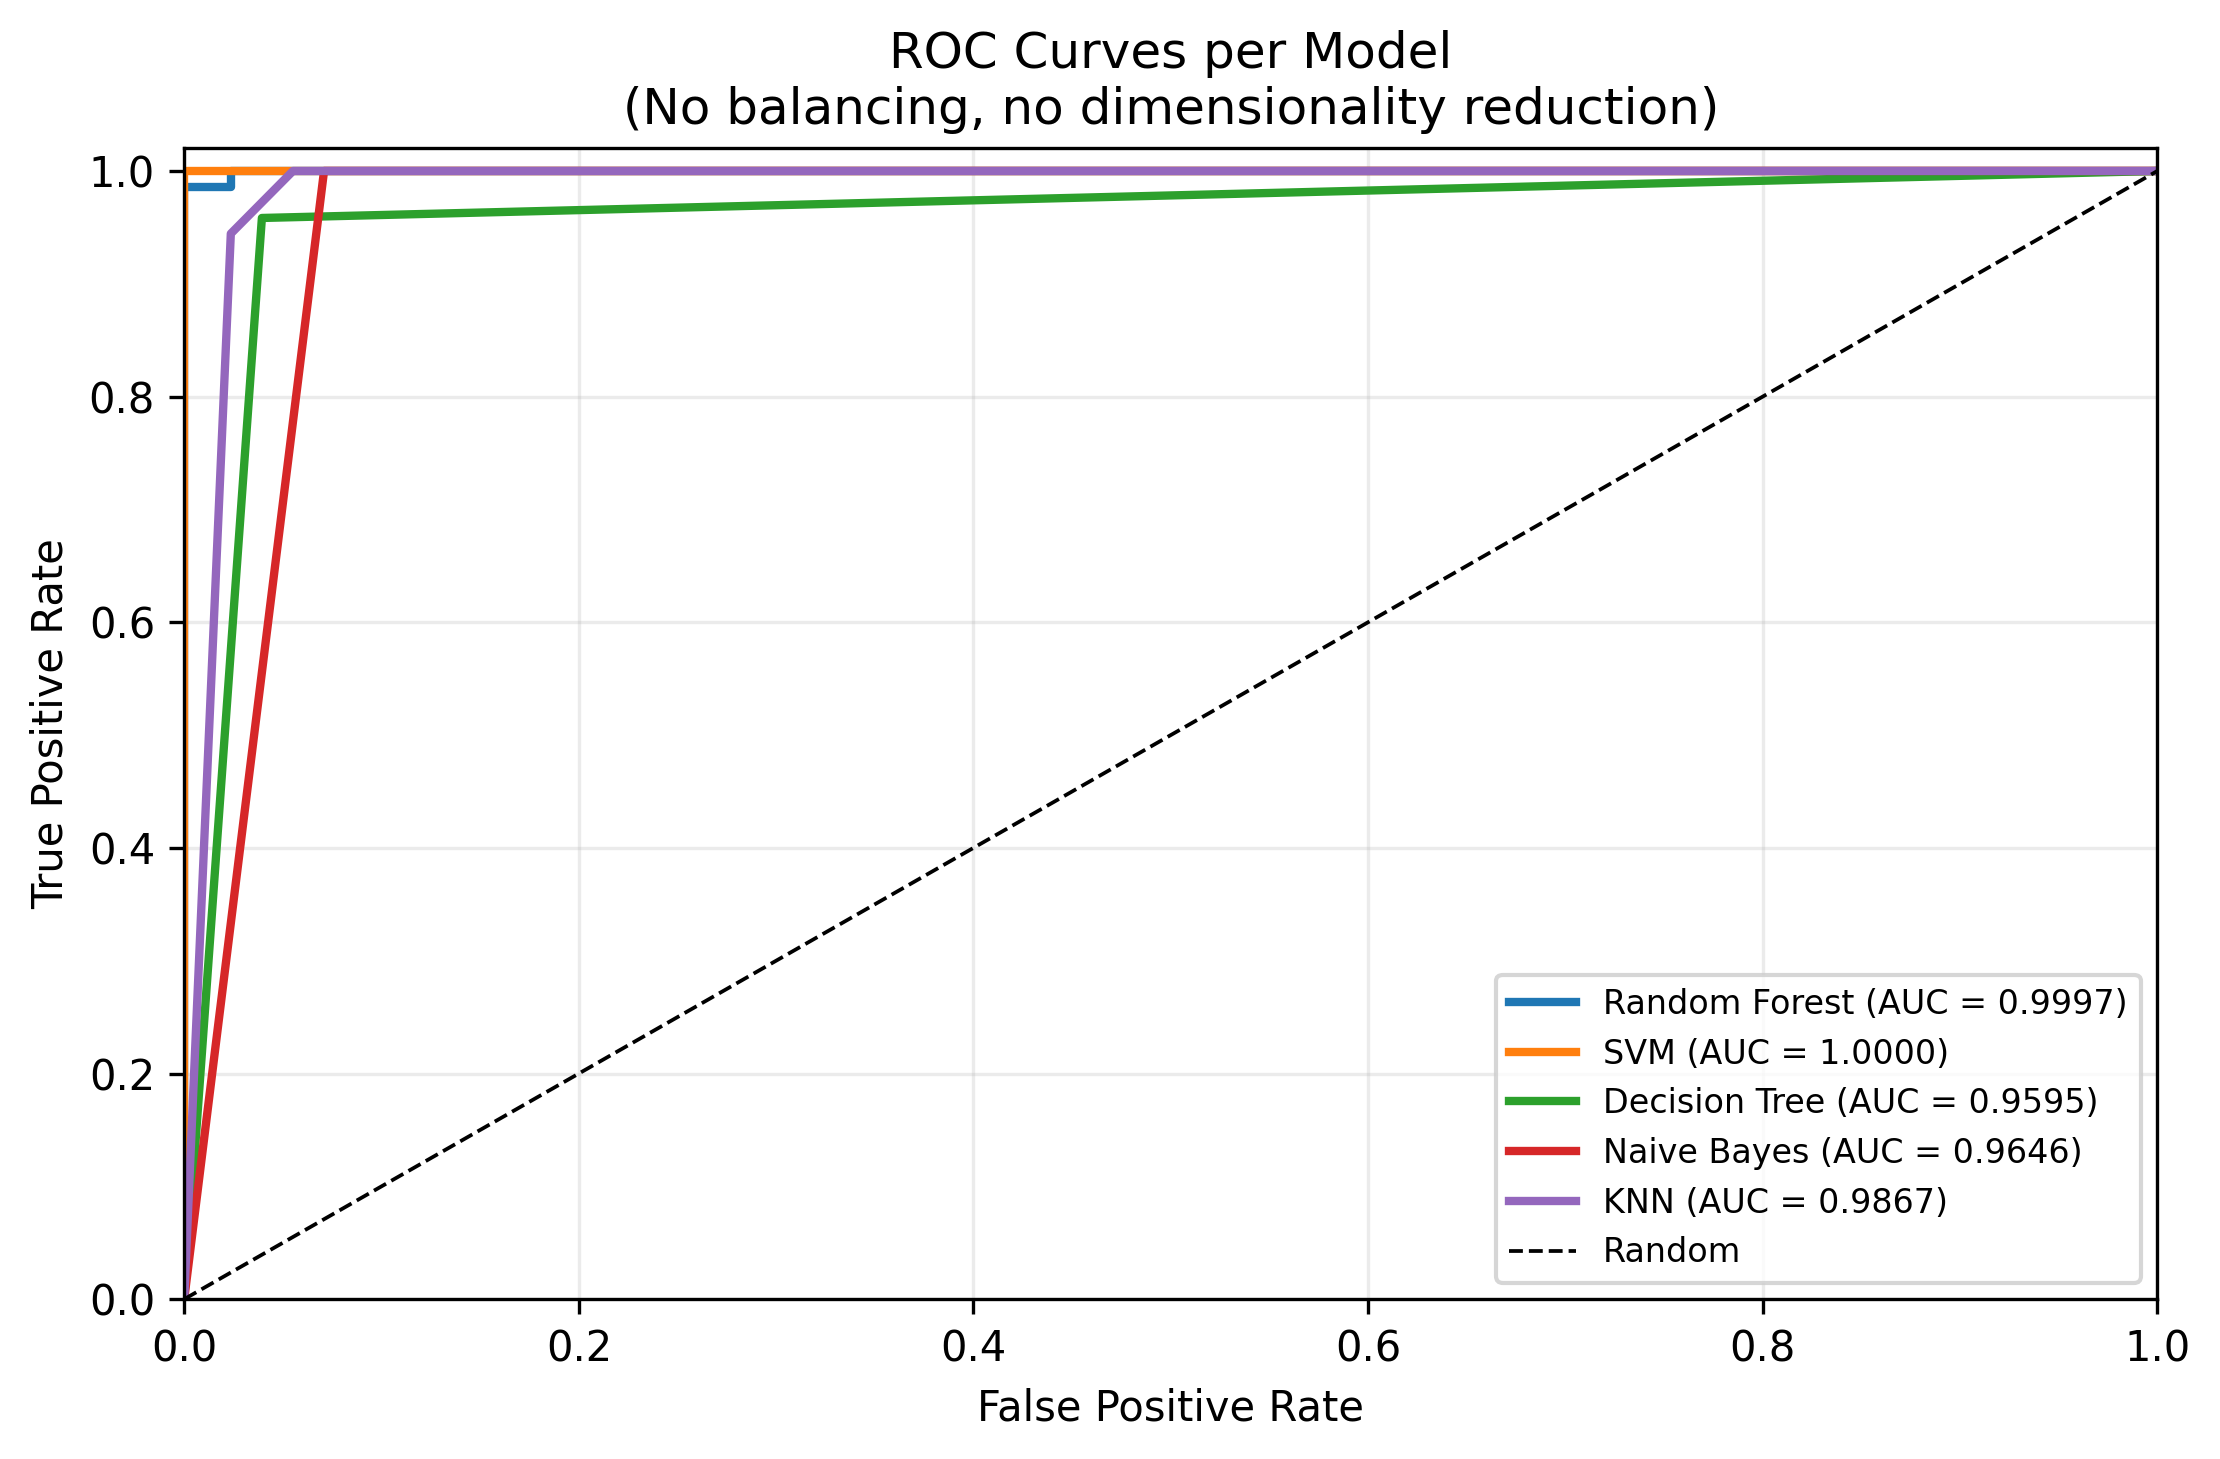
\includegraphics[width=\linewidth]{figures/model_comparison_no_dr_roc_curve.png}
\caption{ROC curves.}
\end{subfigure}
\caption{Initial model-comparison results.}
\label{fig:model_comparison_results}
\end{figure}

\FloatBarrier

\subsection{Balancing and Dimensionality Reduction}

The balancing experiments compared the original class distribution against
SMOTE, Random Under Sampling, and SMOTE combined with Tomek Links. Because the
dataset has only moderate imbalance, the balancing techniques did not improve
the average performance across models. The best average F1-score was obtained
without balancing, with F1-score of 0.9555 across the evaluated algorithms.
For Random Forest specifically, the F1-score remained 0.9926 for no balancing,
SMOTE, and SMOTE with Tomek Links, while Random Under Sampling reduced the
F1-score to 0.9867. Therefore, the final workflow did not include a balancing
step.

\begin{table}[!htbp]
\centering
\caption{Average results by balancing strategy across evaluated models.}
\label{tab:balancing_results}
\begin{tabular}{lcccc}
\hline
Strategy & Accuracy & Precision & Recall & F1-score \\
\hline
No balancing & 0.9658 & 0.9281 & 0.9886 & 0.9555 \\
SMOTE + Tomek Links & 0.9628 & 0.9219 & 0.9886 & 0.9518 \\
SMOTE & 0.9618 & 0.9193 & 0.9886 & 0.9506 \\
Random Under Sampling & 0.9537 & 0.9014 & 0.9914 & 0.9416 \\
\hline
\end{tabular}
\end{table}

Dimensionality-reduction experiments showed that PCA produced the strongest
average performance across the evaluated models. PCA retaining 90\% of the
variance achieved the best average F1-score across classifiers.

For Random Forest, PCA retaining 95\% of the variance produced the highest mean
F1-score. However, the difference from the no-dimensionality-reduction baseline
was only 0.0009. Since this gain was very small and
PCA reduces the direct traceability between model explanations and the original
clinical variables, the final workflow kept the no-PCA configuration.

\begin{table}[!htbp]
\centering
\caption{Random Forest results by dimensionality-reduction strategy.}
\label{tab:rf_dimensionality_reduction}
\begin{tabular}{lcccc}
\hline
Strategy & Accuracy & Precision & Recall & F1-score \\
\hline
PCA 95\% & 0.9950 & 0.9875 & 1.0000 & 0.9935 \\
No dimensionality reduction & 0.9949 & 1.0000 & 0.9857 & 0.9926 \\
PCA 90\% & 0.9900 & 0.9742 & 1.0000 & 0.9867 \\
Filter (mutual information) & 0.9899 & 0.9867 & 0.9857 & 0.9857 \\
Embedded Random Forest & 0.9899 & 0.9867 & 0.9857 & 0.9857 \\
Filter (ANOVA F-test) & 0.9847 & 0.9867 & 0.9714 & 0.9777 \\
Embedded LinearSVC & 0.9797 & 0.9857 & 0.9571 & 0.9703 \\
\hline
\end{tabular}
\end{table}

\begin{table}[!htbp]
\centering
\caption{Average ranking of dimensionality-reduction strategies across evaluated models.}
\label{tab:dr_average_ranking}
\begin{tabular}{lcccc}
\hline
Strategy & Accuracy & Precision & Recall & F1-score \\
\hline
PCA 90\% & 0.9759 & 0.9475 & 0.9914 & 0.9679 \\
PCA 95\% & 0.9749 & 0.9459 & 0.9914 & 0.9669 \\
Embedded Random Forest & 0.9719 & 0.9425 & 0.9886 & 0.9632 \\
Filter (mutual information) & 0.9718 & 0.9398 & 0.9886 & 0.9625 \\
Filter (ANOVA F-test) & 0.9708 & 0.9404 & 0.9857 & 0.9610 \\
No dimensionality reduction & 0.9658 & 0.9281 & 0.9886 & 0.9555 \\
Embedded LinearSVC & 0.9598 & 0.9217 & 0.9802 & 0.9475 \\
\hline
\end{tabular}
\end{table}

\FloatBarrier

\subsection{Hyperparameter Tuning and Final Model}

The Random Forest classifier was further evaluated using default parameters,
GridSearchCV, and RandomizedSearchCV under two preprocessing settings: no
dimensionality reduction and PCA retaining 95\% of the variance. The default
Random Forest configuration refers to the default parameters of the
scikit-learn version used in the experiments.

The tuning results showed that hyperparameter search did not provide a
meaningful gain over the default Random Forest configuration. With PCA 95\%,
GridSearchCV and the baseline configuration reached the same mean F1-score of
0.9935. Without PCA, the baseline, GridSearchCV, and the fine RandomizedSearchCV
configuration also reached the same mean F1-score of 0.9926.

Because the performance difference between the best PCA-based configuration and
the no-PCA Random Forest was only 0.0009 in mean F1-score, the final selected
model was the default Random Forest without balancing and without PCA. This
choice preserves near-identical predictive performance while avoiding the
additional pipeline complexity of PCA and hyperparameter search. It also keeps
the model easier to interpret using the original clinical attributes. The
hyperparameter-tuning ranking is summarized in
Table~\ref{tab:rf_hyperparameter_ranking}, and the supporting plots are shown
in Figure~\ref{fig:rf_hyperparameter_results}.

\begin{table}[!htbp]
\centering
\caption{Random Forest hyperparameter-tuning ranking.}
\label{tab:rf_hyperparameter_ranking}
\resizebox{\linewidth}{!}{%
\begin{tabular}{llcccc}
\hline
Preprocessing & Configuration & Accuracy & Precision & Recall & F1-score \\
\hline
PCA 95\% & GridSearchCV & 0.9950 & 0.9875 & 1.0000 & 0.9935 \\
PCA 95\% & Baseline & 0.9950 & 0.9875 & 1.0000 & 0.9935 \\
No DR & Baseline & 0.9949 & 1.0000 & 0.9857 & 0.9926 \\
No DR & GridSearchCV & 0.9949 & 1.0000 & 0.9857 & 0.9926 \\
No DR & RandomizedSearchCV fine & 0.9949 & 1.0000 & 0.9857 & 0.9926 \\
PCA 95\% & RandomizedSearchCV broad & 0.9900 & 0.9742 & 1.0000 & 0.9867 \\
PCA 95\% & RandomizedSearchCV fine & 0.9900 & 0.9742 & 1.0000 & 0.9867 \\
No DR & RandomizedSearchCV broad & 0.9899 & 0.9875 & 0.9857 & 0.9861 \\
\hline
\end{tabular}
}
\end{table}

\begin{figure}[!htbp]
\centering
\begin{subfigure}{0.48\linewidth}
\centering
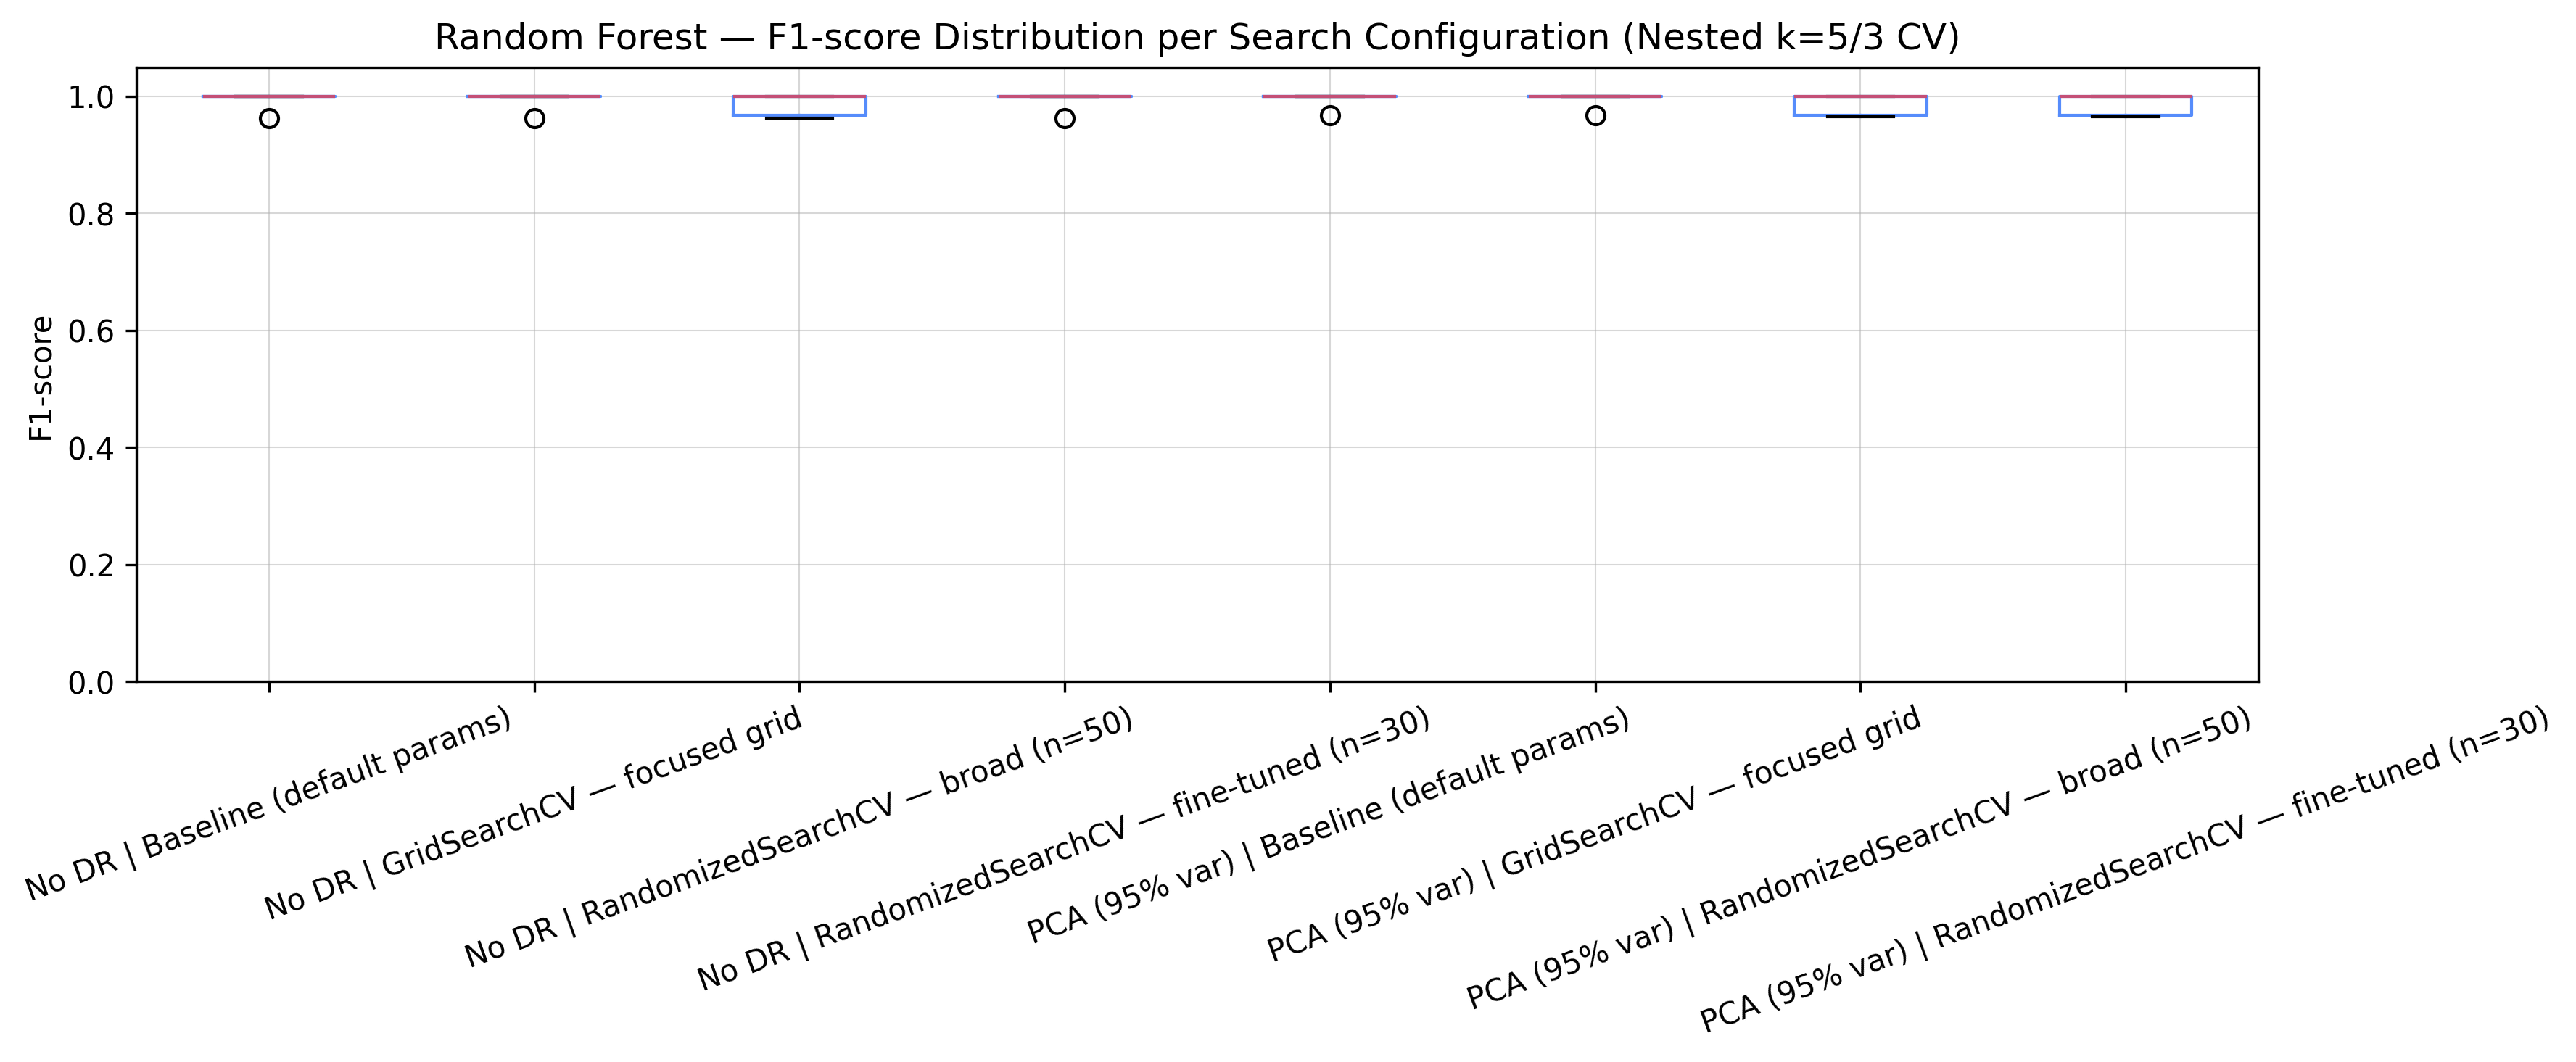
\includegraphics[width=\linewidth]{figures/optimize_rf_hyperparameters_boxplot.png}
\caption{F1-score distribution.}
\end{subfigure}
\hfill
\begin{subfigure}{0.48\linewidth}
\centering
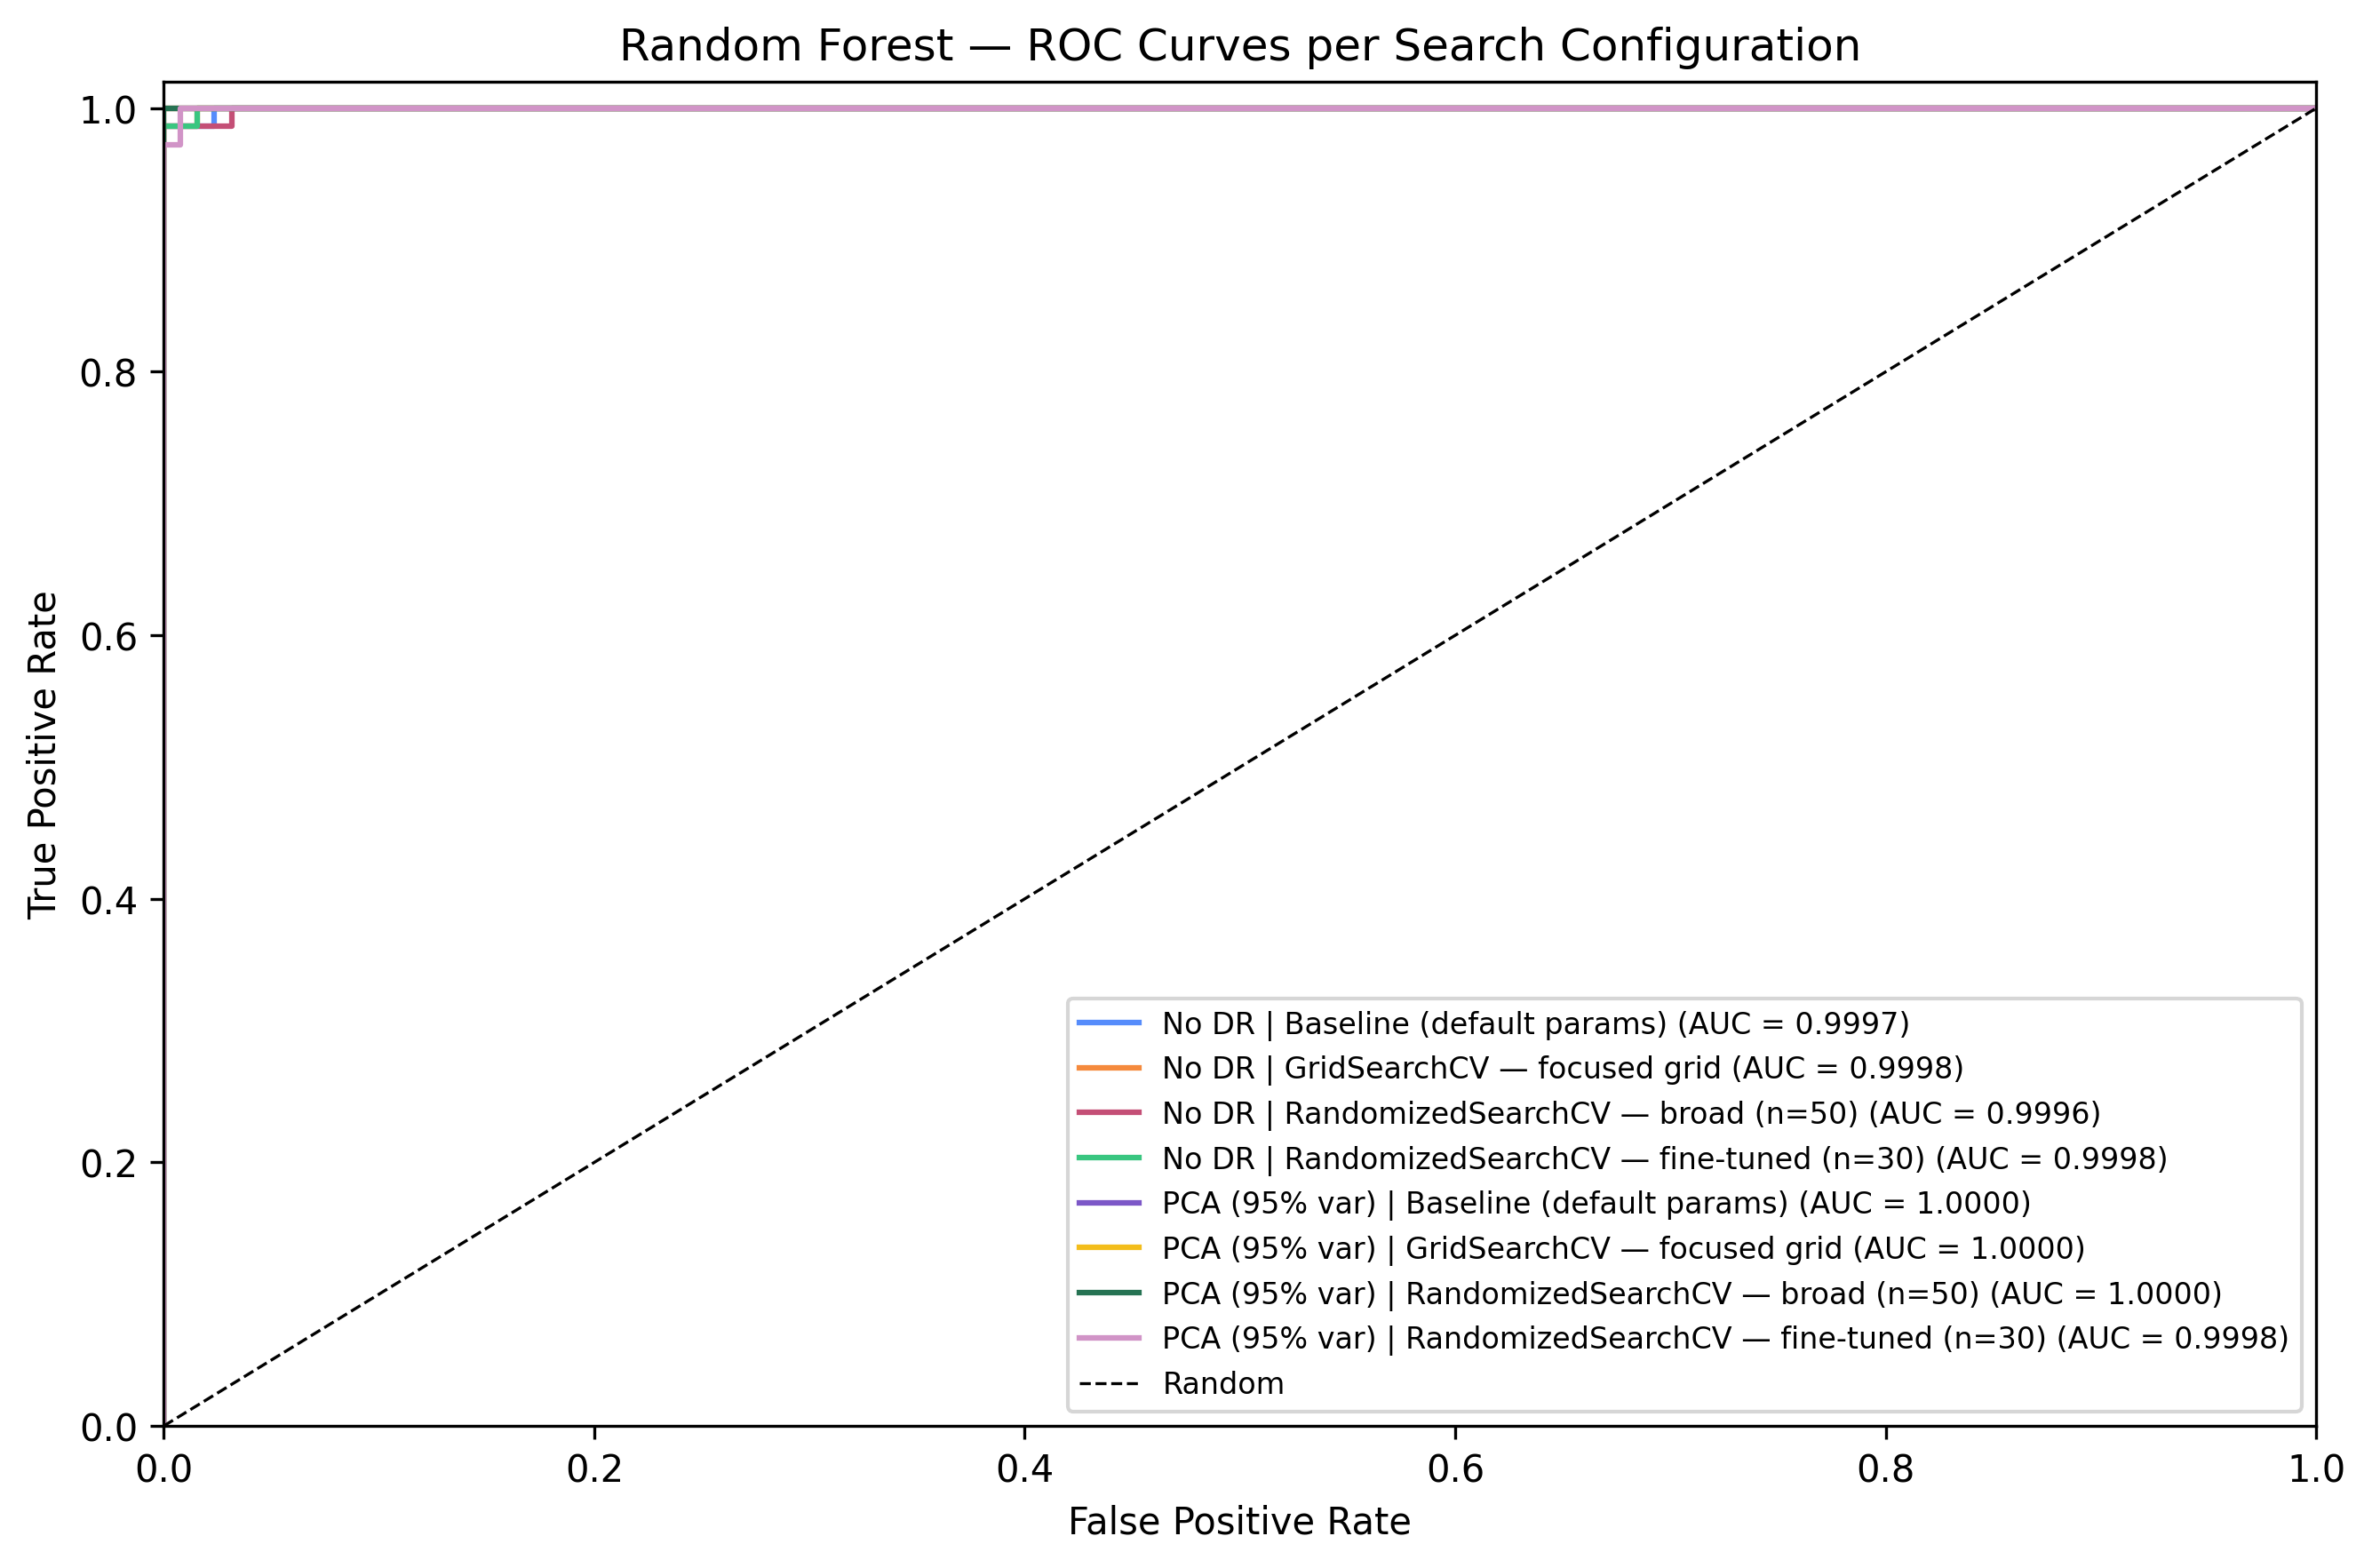
\includegraphics[width=\linewidth]{figures/optimize_rf_hyperparameters_roc_curve.png}
\caption{ROC curves.}
\end{subfigure}
\caption{Random Forest hyperparameter-tuning supporting plots.}
\label{fig:rf_hyperparameter_results}
\end{figure}

\FloatBarrier

\subsection{Explainability and Interpretation Results}

The explainability analysis was applied to the previously selected Random
Forest classifier. The goal of this stage was to interpret the selected model
after model selection, not to introduce a new model-selection criterion. The
analysis focused on the configured explained class \texttt{ckd}, so positive
SHAP values indicate increased support for this class and negative SHAP values
indicate reduced support for this class \cite{lundberg2017shap}.

Global interpretation combined native Random Forest feature importance,
permutation importance, and SHAP summaries. The resulting rankings highlighted
hematological, renal-function, and urine-related variables as relevant features
associated with model predictions. These rankings should be interpreted as
model-dependent predictive patterns rather than causal clinical effects. The
most relevant variables included hematological indicators such as hemo, pcv,
and rbcc; renal and urine-related attributes such as sg, grf, and al; and
clinical indicators such as htn, dm, and bgr. These correspond to hemoglobin,
packed cell volume, red blood cell count, specific gravity, glomerular
filtration rate, albumin, hypertension, diabetes mellitus, and blood glucose
random. Figure~\ref{fig:global_feature_importance_comparison} compares the
native feature-importance and permutation-importance views.

\begin{figure}[!htbp]
\centering
\begin{subfigure}{0.48\linewidth}
\centering
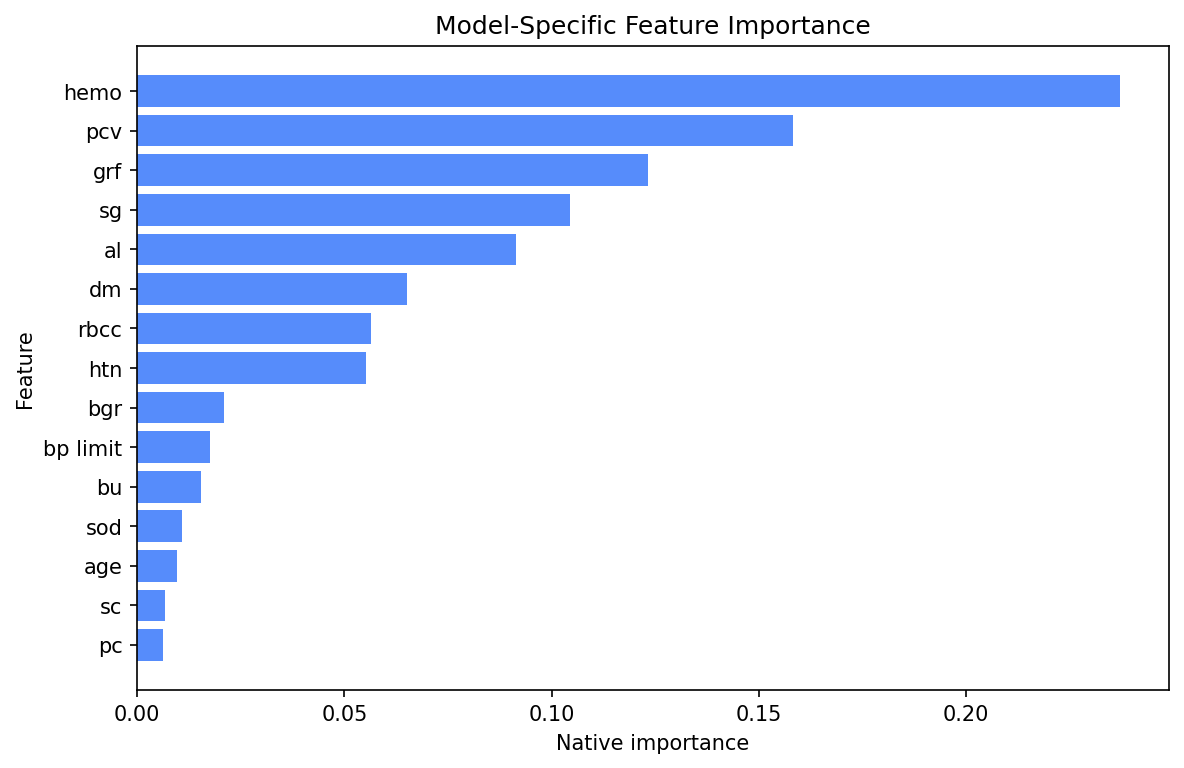
\includegraphics[width=\linewidth]{figures/native_feature_importance.png}
\caption{Model-specific feature importance.}
\label{fig:explainability_native_importance}
\end{subfigure}
\hfill
\begin{subfigure}{0.48\linewidth}
\centering
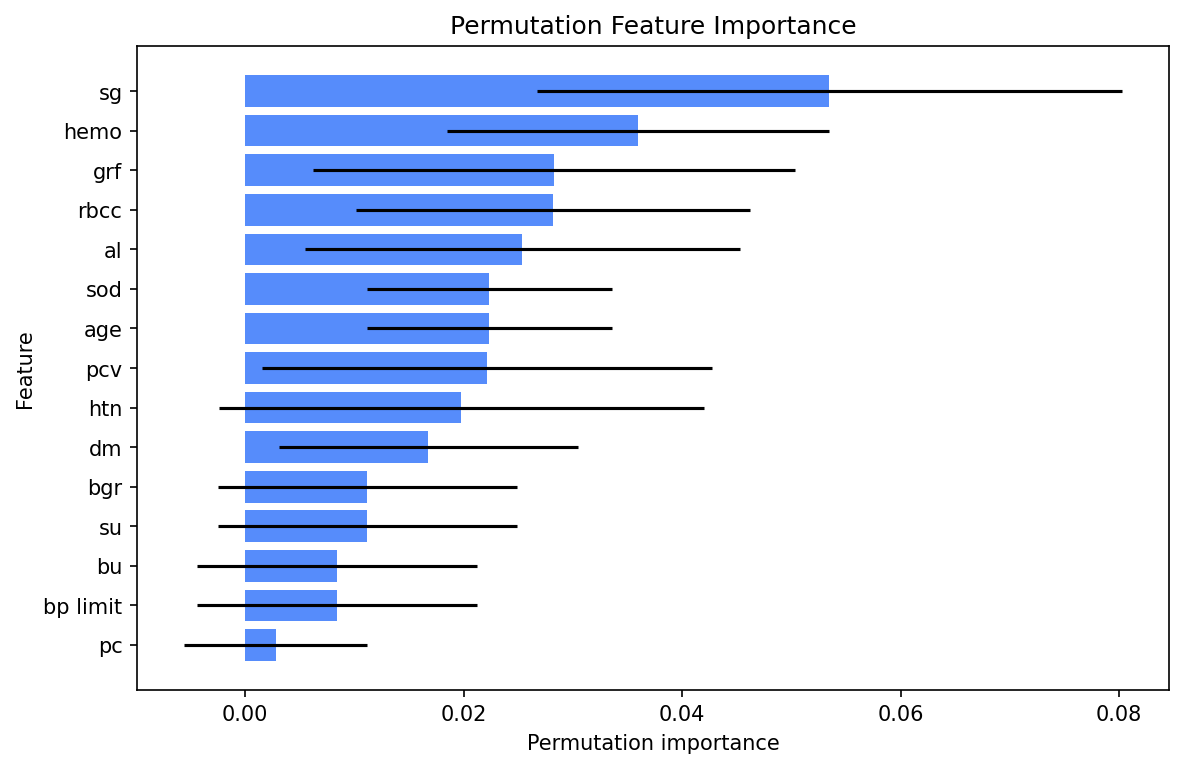
\includegraphics[width=\linewidth]{figures/permutation_importance.png}
\caption{Permutation feature importance.}
\label{fig:explainability_permutation_importance}
\end{subfigure}
\caption{Global feature-importance analysis for the selected Random Forest classifier.}
\label{fig:global_feature_importance_comparison}
\end{figure}

\FloatBarrier

SHAP summaries provided a complementary global interpretation of the selected
classifier. Figure~\ref{fig:global_shap_explanations} reports the mean absolute
SHAP values and the SHAP beeswarm summary for the explained class
\texttt{ckd} \cite{doshivelez2017interpretable,lundberg2017shap}.

\begin{figure}[!htbp]
\centering
\begin{subfigure}{0.48\linewidth}
\centering
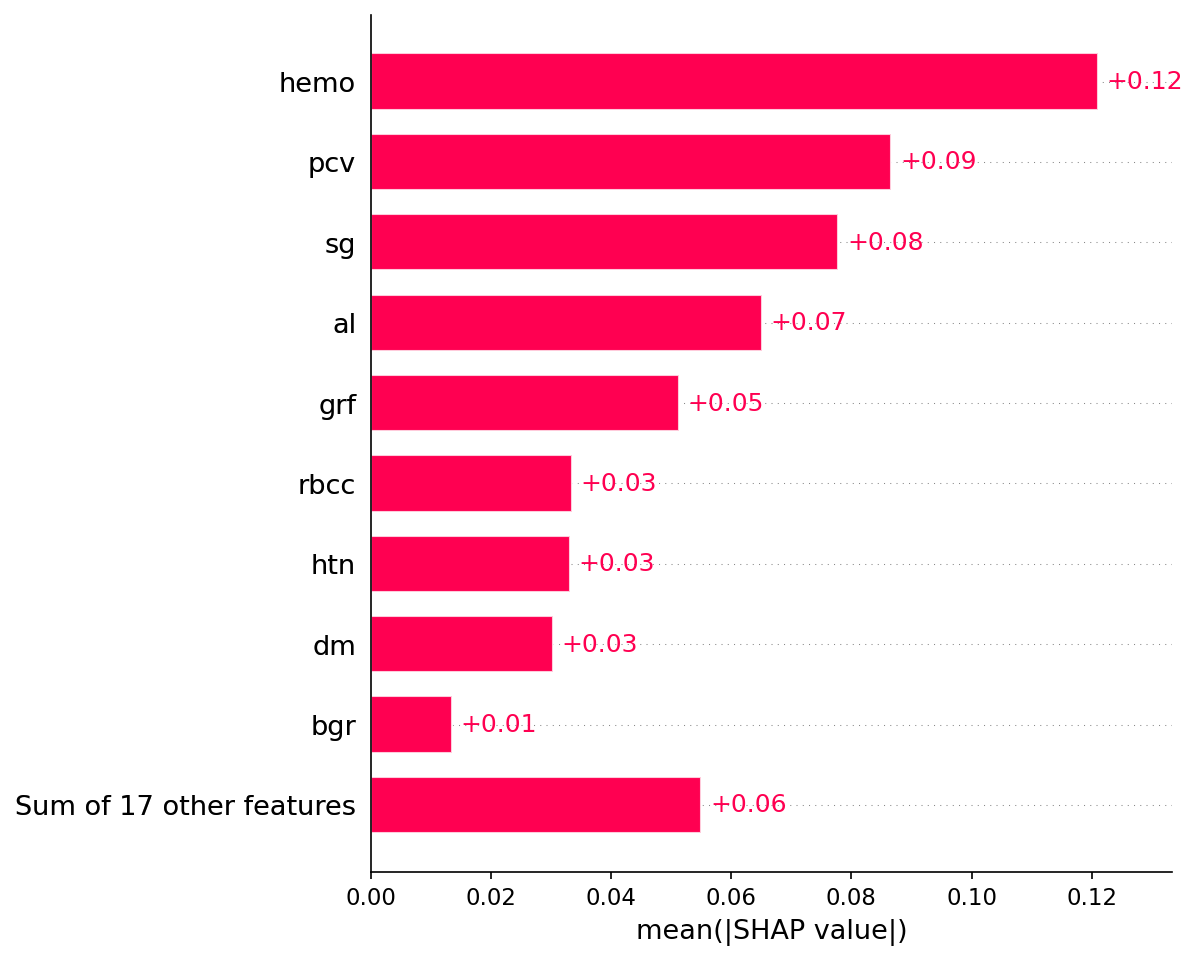
\includegraphics[width=\linewidth]{figures/shap_global_bar.png}
\caption{Mean absolute SHAP values.}
\label{fig:explainability_shap_global_bar}
\end{subfigure}
\hfill
\begin{subfigure}{0.48\linewidth}
\centering
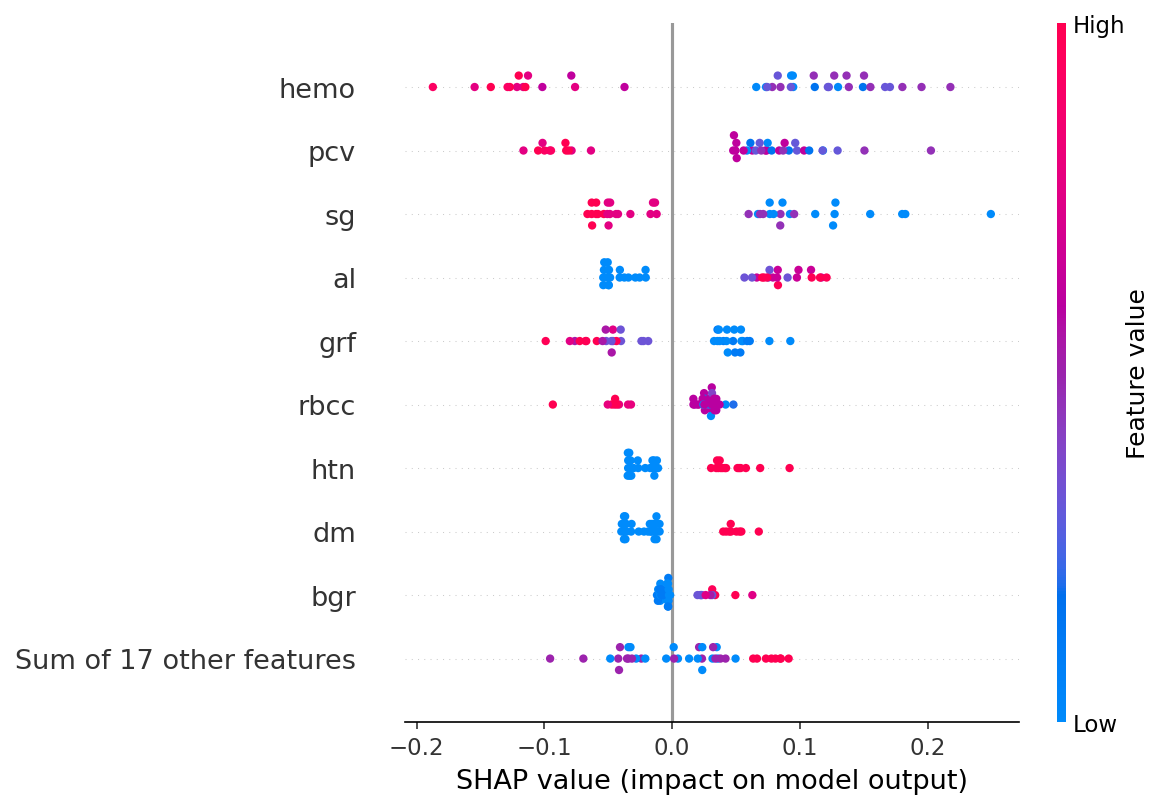
\includegraphics[width=\linewidth]{figures/shap_beeswarm.png}
\caption{SHAP beeswarm summary.}
\label{fig:explainability_shap_beeswarm}
\end{subfigure}
\caption{Global SHAP explanations for the configured explained class, \texttt{ckd}.}
\label{fig:global_shap_explanations}
\end{figure}

\FloatBarrier

Local explanations were generated for representative test instances using SHAP
waterfall plots and LIME. The LIME outputs were exported as local HTML and CSV
artifacts and used as complementary local explanations
\cite{ribeiro2016lime}. Figure~\ref{fig:local_shap_waterfall_explanations}
shows the local SHAP waterfall explanations included in the paper.

\begin{figure}[!htbp]
\centering
\begin{subfigure}{0.46\linewidth}
\centering
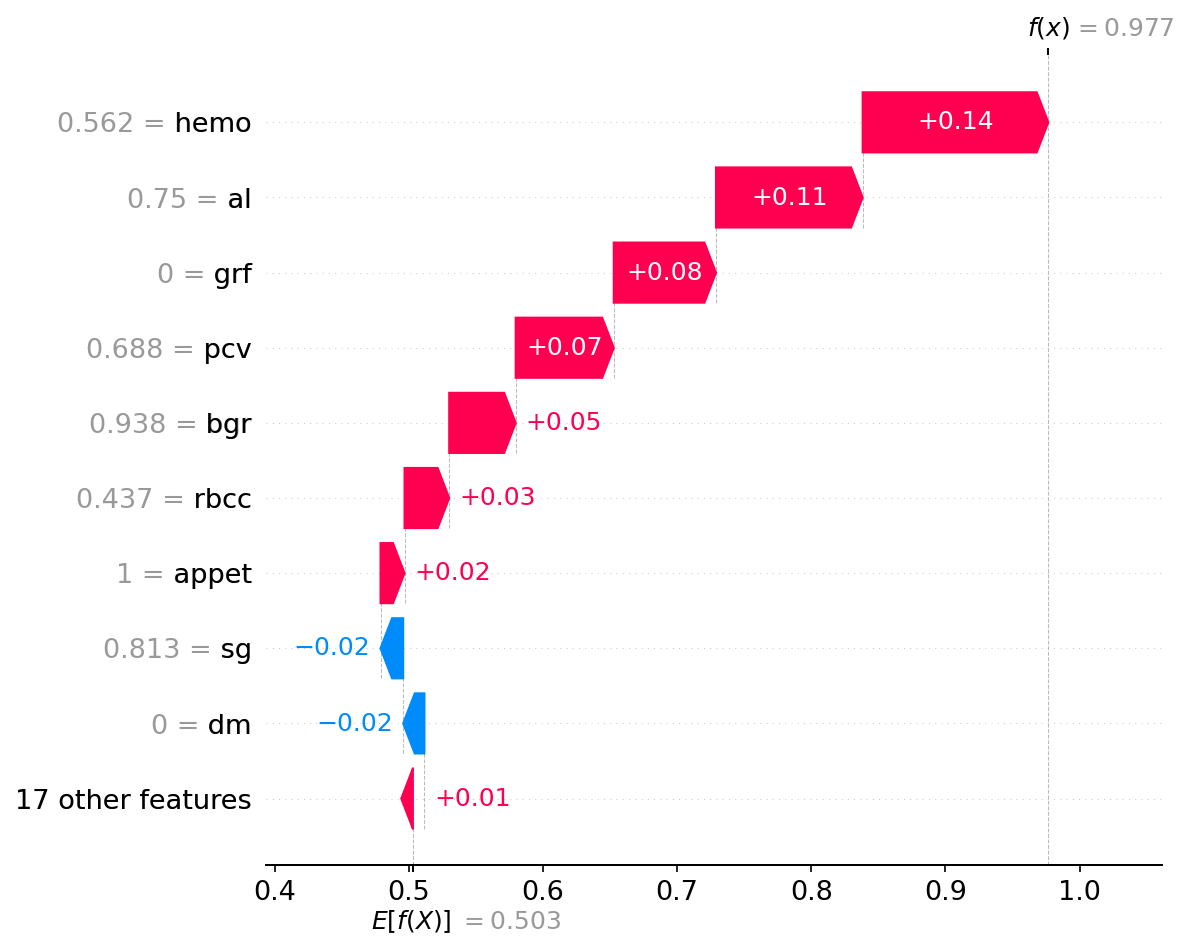
\includegraphics[width=\linewidth]{figures/shap_waterfall_instance_0.png}
\caption{Representative instance.}
\label{fig:explainability_shap_waterfall_instance_0}
\end{subfigure}
\hfill
\begin{subfigure}{0.46\linewidth}
\centering
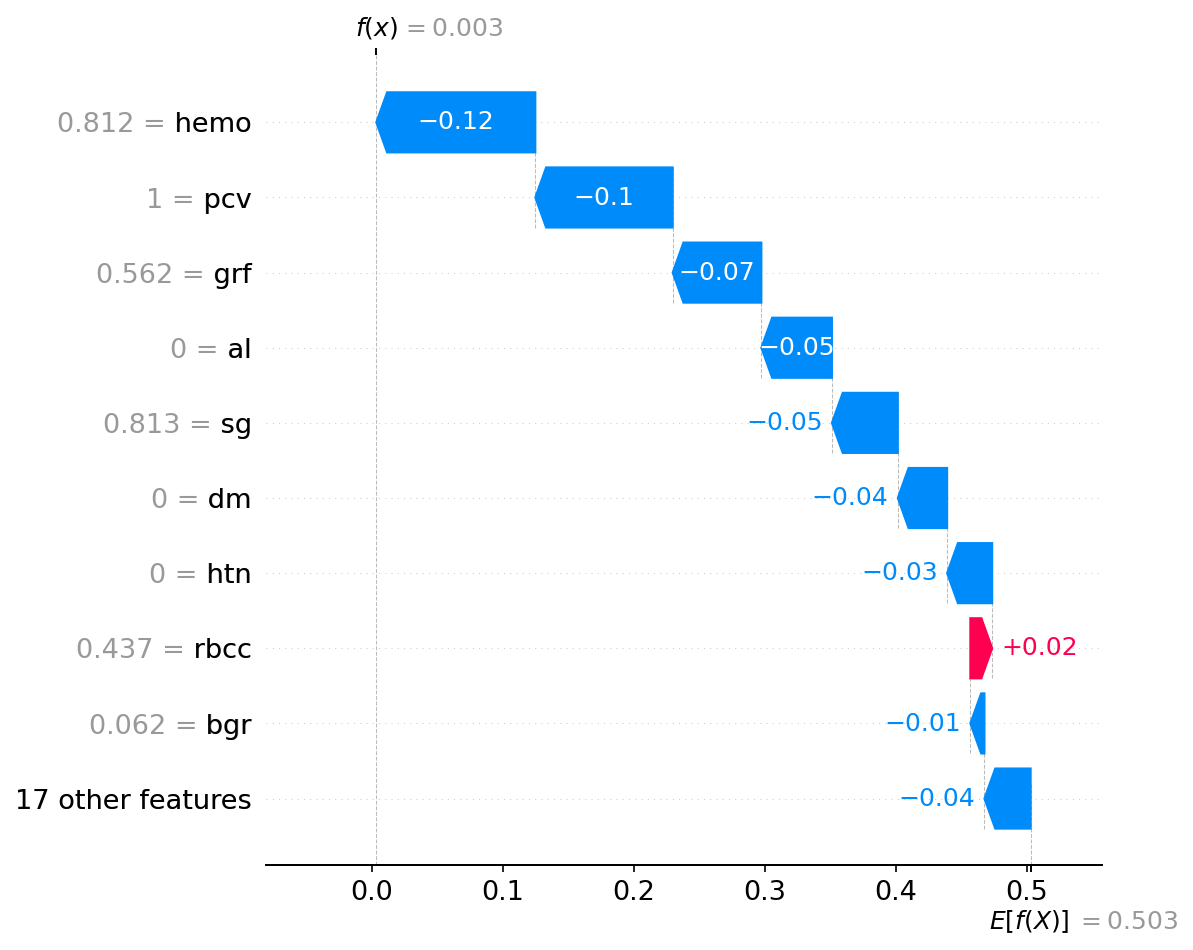
\includegraphics[width=\linewidth]{figures/shap_waterfall_instance_4.png}
\caption{Second representative instance.}
\label{fig:explainability_shap_waterfall_instance_4}
\end{subfigure}
\caption{Local SHAP waterfall explanations for representative test instances.}
\label{fig:local_shap_waterfall_explanations}
\end{figure}

\FloatBarrier
